\section{Description technique}

Comme cité précédemment, notre application a été codé à l'aide de la librairie JavaFX. Ainsi, toute notre implémentation technique est basée sur cette dernière. 

\subsection{Structure}
JavaFX utilise des fichiers FXML pour séparer la logique de la vue TODO TODO TODO
ImageView, Canvas et Text
Controller

\subsection{Serialisation}
En Java, la sérialisation s'effectue à l'aide de l'interface \og Serializable \fg{}. Par conséquent, chaque classes de Java implémentant cette dernière telle que \og String \fg{}, peut être sérialisé et désérialisé à volonté. Cependant, la majorité des classes JavaFX n'implémente pas cette interface. En effet, cette librairie utilise grandement des mécanismes et des liaisons dynamiques tel que les listeners qui sont pour l'instant des sous-systèmes non-sérialisable. C'est pourquoi, JavaFX contient peu d'objet sérialisable.

Pour combler ce manque, nous devons nous même implémenter la sérialisation des classes JavaFX que nous sommes susceptible d'utiliser. 

\begin{figure}[h]
    \caption{Diagramme de la sérialisation simplifié}
    \centering
    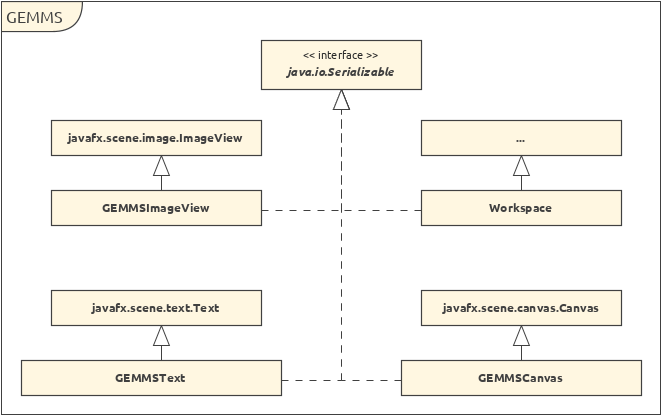
\includegraphics[scale=0.6]{serialisation_diagram.png}
    \label{fig:seri_diag}
\end{figure}

Sur la figure \ref{fig:seri_diag}, nous pouvons voir un diagramme simplifié de l'implémentation de la sérialisation. Dans notre application, nous allons utilisé des classes de base telles que ImageView, Text, Canvas, Color, etc. Nous devons donc spécialiser ces classes afin qu'elles puissent implémenter l'interface \og Serializable \fg{}. Toutefois, certaines classes comme \og Color \fg{} ne sont malheureusement pas spécialisable. Il faut donc sérialiser les paramètres un par un à l'aide des accesseurs et mutateurs de cette dernière.

Étant donné que les classes JavaFX possèdent énormément de fonctionnalités, sérialiser l'entier de celles-ci nous demanderait beaucoup trop de temps. C'est pourquoi nous nous contentons uniquement des paramètres utilisés au sein du projet tel que la largeur, la hauteur, la position, etc. 

\lstinputlisting[language=Java, caption=Exemple de sérialisation]{./src/serialisation.java}

Bien que la sérialisation soit possible, ceci engendre des contraintes et des pertes de performances. Par exemple, les classes spécialisées ne peuvent plus étendre d'une classe commune et bénéficier de ses méthodes. De plus, les objets comme Canvas et ImageView devront sérialiser pixel par pixel, ce qui peut être long et volumineux selon la taille.

\subsection{Sauvegarde}
La sauvegarde d'un document utilise la sérialisation des objets. Comme mentionné précédemment, la sérialisation de certaines classes peut être volumineux. Ainsi, les données sont compressées dans le format GZIP.

\subsection{Workspace et liste des calques}
TODO TODO TODO

\subsection{Copier-coller}
TODO TODO TODO

\subsection{Historique}
Pour garder un historique de chaque action effectuée, on utilise la sérialisation des composants présentée précédemment. A la fin de chaque action modifiant l'espace de travail, une fonction va être appelée permettant de sauvegarder intégralement l'espace de travail courant et le placer sur une pile. A chaque détection de la commande Ctrl + Z, la sauvegarde sera chargée et la modification sera donc effacée. De même, à la détection de la commande Ctrl + Y, on va charger un espace de travail plus récent (s'il y en à un, c'est-à-dire si le Ctrl + Y était précédé d'un Ctrl + Z).

\subsection{Positionnement}
TODO TODO TODO

\subsection{Outils}
\par
JavaFX offre (entre autres) les événements MousePressed, MouseDragged et MouseReleased. Ils correspondent respectivement à l'action de presser la souris, de la déplacer en gardant le clic gauche enfoncé ou de relâcher le clic gauche de la souris. 
\subsubsection{Hiérarchie des outils}
\par
La plupart des outils de l'application  fonctionnent grâce à ces trois événements. On pensera notamment au pinceau qui doit dessiner un trait en suivant la souris lors d'un MouseDragged. 
\par
Comme on peut le voir sur la figure \ref{fig:tool_hier}, les outils implémentent donc une interface Tool, possédant des méthodes correspondant à ces événements. Au long de l'exécution du programme, le Workspace garde une référence vers un outil considéré actif (qui peut aussi être référence nulle), et lorsqu'il détecte un des événements cités plus haut, il se charge d'appeler la ou les méthodes correspondantes de cet outil.
\par

\begin{figure}[h]
	\caption{Diagramme simplifié de la hiérarchie des outils}
	\centering
	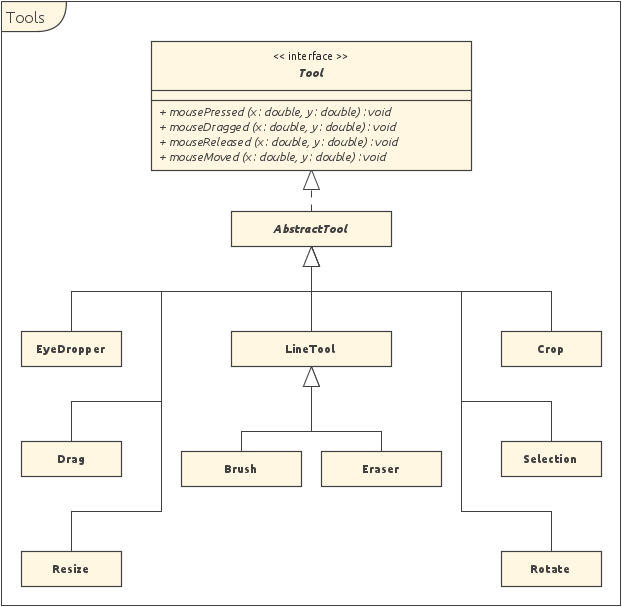
\includegraphics[scale=0.6]{tool_hierarchy.png}
	\label{fig:tool_hier}
\end{figure}

\subsubsection{Réglage des outils}
Certains de ces outils nécessitent d'être paramétrés en temps réel en fonction des calques sélectionnés par l'utilisateur. Par exemple, la taille de la gomme est stockée dans l'objet représentant l'outil, et est utilisée pour déterminer la taille du rectangle à effacer. L'utilisateur peut la régler au moyen d'un Slider (il s'agit d'un composant JavaFX). Les même besoin concernent la gestion de la couleur du pinceau, de la taille et de la police de l'outil de modification de texte.
\par
Ces réglages sont gérés au moyen d'une hiérarchie de classes, qui sont en fait des spécialisations de composant JavaFX permettant à l'utilisateur de paramétrer les outils, et d'une série d'interfaces représentant des outils pouvant être paramétrés sur divers aspects (la taille, la couleur, la police et ainsi de suite).
\par
TODO ajouter schéma
\subsubsection{Pinceau et gomme}
Le pinceau et la gomme ont un comportement et une implémentation quasiment identiques. Dans le programme GEMMS, ce sont les classes Brush et Eraser qui se chargent d'implémenter ces fonctionnalités. Toutes deux héritent d'une classe commune: LineTool. 
\par
Pour ces deux outils, la problématique était la suivante: 
\par 
L'événement MouseDragged est déclenché à intervalles réguliers, tant que l'utilisateur effectue cette action. Pour chaque répétition, il est facile de garder trace de la position de la souris au dernier événement et à l'événement actuel. Connaissant ces deux points, il est possible de dessiner une droite.
\par
Pour ce faire, nous avons utilisé l'algorithme de tracé de segment de Bresenham. Mis au point en 1962, cet algorithme permet de déterminer quels pixels sont à colorer pour relier harmonieusement deux points par une ligne droite.
\par
Il existe de nombreuses implémentations de cet algorithme, et nous avons choisi l'implémentation compacte, que l'on peut trouver sur la page allemande de l'article Wikipédia dédié à ce sujet \cite{Bresenham}.
\par
La classe LineTool se charge donc d'implémenter cet algorithme et pour chaque pixel à colorer, elle appelle une méthode abstraite drawPixel que ses sous classes se chargent de définir. Ainsi, Brush dessiner un disque correspondant à la taille du pinceau, et Eraser efface un carré de pixel, correspondant à la taille de la gomme.
\subsubsection{Pipette}
Le rôle de l'outil pipette et de permettre à l'utilisateur de choisir une couleur en la prélevant sur un élément existant du document. Il s'agirait typiquement de récupérer la couleur d'un calque GEMMSText, GEMMSCanvas ou GEMMSImage.
\par 
Dans le cas d'un texte, la pipette retourne simplement la couleur de celui-ci. Dans le cas d'un objet de type GEMMSCanvas ou d'une GEMMSImage, l'outil lit le pixel exact cliqué par l'utilisateur, ci celui-ci se trouve à l'intérieur des bornes du calque sélectionné.
\subsubsection{Modification de texte}
L'outil de modification de texte permet à l'utilisateur de modifier les propriétés d'un calque texte existant. Lorsque cet outil est activé
\subsubsection{Symétries}
\subsubsection{Déplacement}
\subsubsection{Rotation}
\subsubsection{Redimensionnement}
\subsubsection{Sélection}
\subsubsection{Rognage}



